\chapter{Base de datos y funcionamiento sin conexión}
\label{cap:datos}

La persistencia remota de la información y una interfaz web que simplificara la administración de los usuarios se definieron como funcionalidades complementarias al MVP. Su implementación quedó condicionada al tiempo disponible luego de completar y validar el núcleo principal del sistema. Este capítulo describe cómo se resolvieron, junto con los mecanismos que permiten que el sistema siga funcionando cuando no hay conexión a Internet.

\section{Arquitectura de persistencia con Supabase}

Para esta etapa se utilizó el plan gratuito de Supabase, una plataforma que proporciona una base de datos PostgreSQL, almacenamiento de archivos y una API para acceder a los recursos del proyecto. En SmartGate, este servicio actúa como repositorio central: conserva los datos de las personas habilitadas, las representaciones faciales asociadas y los registros de acceso. Además, permite almacenar y recuperar las imágenes cargadas por los usuarios, manteniendo una copia persistente de la información disponible aun cuando la Raspberry Pi se reinicie o se encuentre temporalmente fuera de servicio.

La separación de la información en tablas facilita su mantenimiento. La tabla de personas contiene los datos identificatorios y el estado de habilitación; los vectores o características faciales se conservan de forma independiente; y los eventos generados por el sistema quedan registrados para su posterior consulta. Esta organización evita duplicaciones, mejora la trazabilidad y permite ampliar el sistema sin modificar la lógica principal de reconocimiento.

\section{Conexión con la Raspberry Pi}

La Raspberry Pi ejecuta el programa principal de SmartGate y se comunica con Supabase a través de su API mediante una conexión HTTPS. Al iniciarse, el software utiliza la dirección del proyecto y las credenciales configuradas localmente para consultar los usuarios habilitados y obtener las imágenes o representaciones faciales necesarias. Estos datos se descargan y quedan disponibles para el proceso de reconocimiento que se ejecuta en el dispositivo.

Durante el funcionamiento, la Raspberry Pi compara el rostro detectado con la información recuperada desde la base de datos. Si encuentra una coincidencia válida y el usuario está habilitado, la lógica del sistema continúa con la decisión de apertura. A su vez, los resultados de cada intento pueden enviarse nuevamente a Supabase como registros de acceso.

De este modo, la comunicación es bidireccional: la Raspberry Pi consume la información necesaria para reconocer a los usuarios y la base de datos recibe los eventos producidos por el sistema, tal como se muestra en la figura~\ref{fig:interaccion}.

\section{Interfaz web de administración}

Además de la base de datos, se desarrolló con asistencia de ChatGPT una interfaz web de administración. Su objetivo es ofrecer una capa visual sencilla para dar de alta o modificar usuarios, cargar imágenes y consultar los registros almacenados.

De esta manera, las tareas habituales pueden realizarse desde el navegador sin escribir consultas SQL ni ejecutar código, lo que reduce la posibilidad de errores y facilita el uso por parte de personas sin conocimientos técnicos.

La interfaz web presenta la información de forma centralizada. Desde el panel de control es posible consultar la cantidad de personas habilitadas, los accesos autorizados y rechazados, los eventos recientes y el estado general de los servicios. También se muestra explícitamente la conexión con Supabase, lo que facilita distinguir un problema de conectividad de una falla del pipeline local.

\begin{figure}[H]
    \centering
    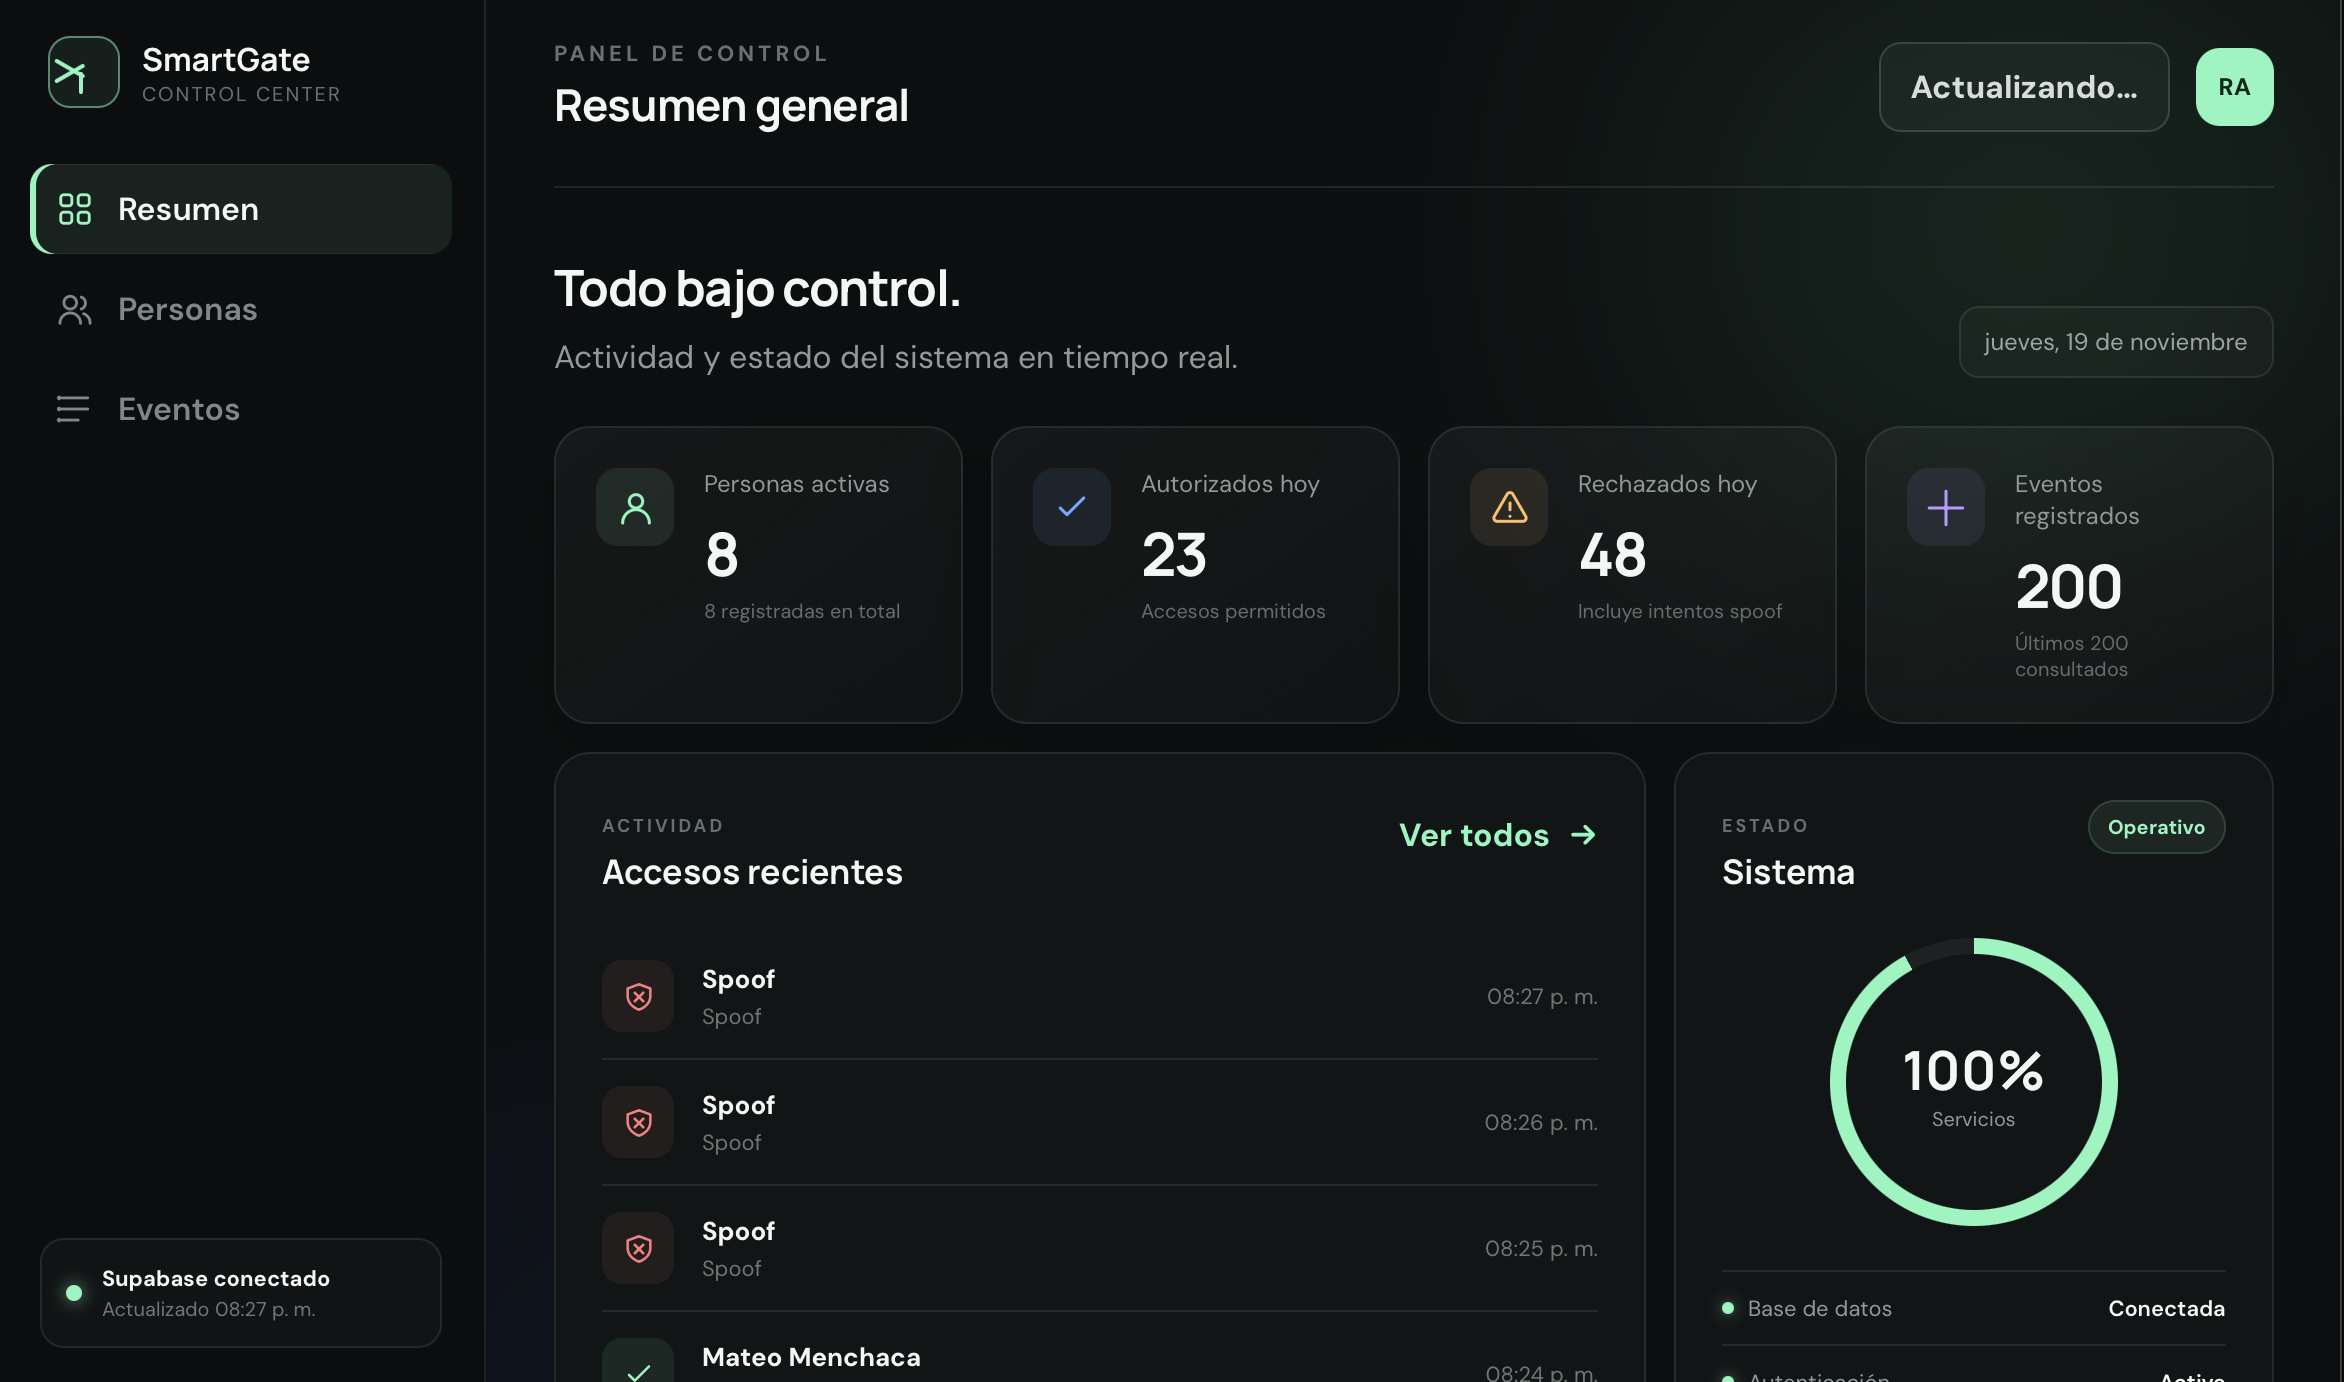
\includegraphics[width=\textwidth]{Imagenes/panel_web.png}
    \caption{Panel web de administración y supervisión conectado a Supabase.}
    \label{fig:panel-web}
\end{figure}

La vista de eventos permite revisar rápidamente resultados autorizados, rechazados y clasificados como spoof. De esta manera, Supabase no solamente cumple una función de almacenamiento, sino que también aporta trazabilidad y una capa de supervisión para evaluar el comportamiento del sistema durante las pruebas.

Como criterio de seguridad, las claves privadas de acceso no deben incorporarse al código visible de la interfaz web. Estas credenciales deben mantenerse en la Raspberry Pi o en un servicio de servidor, mientras que la aplicación web debe operar únicamente con permisos limitados y las políticas de acceso definidas en Supabase.

\section{Funcionamiento sin conexión}
\label{sec:offline}

La conectividad con Supabase se ejecuta en hilos independientes y nunca forma parte del camino crítico de autorización. Por esta razón, una red lenta o la ausencia de Wi-Fi no detienen la cámara, los modelos ni el control GPIO. Para que el reconocimiento pueda continuar, el sistema mantiene en la tarjeta de la Raspberry una copia de la última galería facial válida.

\subsection{Galería facial local}

Aunque habitualmente se la denomina caché de imágenes, el archivo local no conserva las fotografías completas. Durante la sincronización, las imágenes alojadas en Supabase se descargan, se validan y se transforman en embeddings de 128 valores. El respaldo \texttt{data/galeria\_rostros.npz} almacena de forma compacta el identificador, el nombre y los embeddings de cada persona habilitada. Esta representación es suficiente para realizar las comparaciones de SFace y reduce tanto el espacio utilizado como el tiempo de carga.

Al comenzar el reconocimiento, el programa carga primero esta galería desde el disco, antes de intentar comunicarse con Supabase. Por lo tanto, si la placa arranca sin Wi-Fi puede reconocer inmediatamente a los usuarios incluidos en la última sincronización. En paralelo, el worker de galería intenta recuperar la conexión cada diez segundos. Cuando Supabase vuelve a estar disponible, obtiene las personas activas y sus embeddings, compara la nueva galería con la existente y solamente escribe el archivo si hubo cambios.

El guardado de la galería se realiza de forma atómica: se genera un archivo temporal, se fuerza su escritura en la tarjeta y finalmente se reemplaza la versión anterior. De este modo, un corte de alimentación durante la actualización no debería dejar un respaldo incompleto. Además, la galería compartida en memoria se protege mediante un \texttt{Lock}, por lo que puede actualizarse sin interrumpir un reconocimiento que ya se encuentre en curso.

Durante el modo sin conexión se cumplen las siguientes condiciones:

\begin{itemize}
    \item Los usuarios presentes en la última galería sincronizada pueden continuar ingresando.
    \item Las altas, bajas, cambios de habilitación y fotografías nuevas no se reciben hasta recuperar la conexión.
    \item El funcionamiento offline requiere que haya existido al menos una sincronización válida anterior.
    \item Si no existe una galería local, el pipeline puede ejecutarse, pero no tendrá identidades contra las cuales comparar el rostro.
\end{itemize}

\subsection{Persistencia de los eventos de acceso}
\label{sec:eventos}

Los resultados autorizados, rechazados o clasificados como spoof se colocan en una cola en memoria para que el Pipeline Manager pueda continuar sin esperar una respuesta de Internet. Un worker separado intenta insertarlos en la tabla \texttt{access\_events}. Si el envío falla, cada evento se agrega como una línea JSON al archivo \texttt{data/eventos\_pendientes.jsonl}.

Mientras la placa permanezca desconectada, los eventos se acumulan en ese archivo. El worker vuelve a intentar la conexión periódicamente y, cuando la recupera, envía primero los eventos antiguos respetando su orden y después los nuevos. Los registros confirmados se eliminan del respaldo local; si una transferencia vuelve a fallar, se conserva el evento problemático junto con todos los posteriores. Así se mantiene la trazabilidad sin bloquear la decisión de acceso.

En conjunto, esta estrategia combina procesamiento local, caché persistente y sincronización diferida. Supabase permite administrar usuarios y centralizar los registros, pero la operación física del portón permanece disponible aun frente a una interrupción temporal de la red.
